\subsection{Scenario 1: Operational Baseline Behaviour}
\subsubsection{Introduction and Objectives}
Scenario 1 serves as the control environment for the entirety of the experimental phase. In this scenario, the smart home network operates under standard, benign conditions without any external interference or malicious activity from the attacker node. The primary objective is to establish a verifiable "ground truth" of the network's behavior. The scenario goals in detail are the following:

\begin{enumerate}
	\item Generate realistic, benign background traffic that strictly adheres to the Manufacturer Usage Description (MUD) profiles defined previously in Table \ref{table:camera_mud} (Smart Camera) and Table \ref{table:thermostat_mud} (Smart Thermostat).
	\item Capture the raw network interactions during standard operational states such as device data transmission, time synchronization, and periodic telemetry reporting.
	\item Extract and catalogue baseline network metadata. This includes metrics such as flow durations, expected packet lengths, and Inter-Arrival Times (IAT)—to, with the objective to use them as the definitive reference point for anomaly detection in subsequent attack scenarios.
\end{enumerate}


\subsubsection{Expected Behaviour and Theoretical Baselines}

To ensure statistical significance and provide a robust dataset for feature extraction, the Scenario 1 baseline simulation was parameterized for a continuous 1200 seconds (20-minute) capture period. Operating under ideal, interference-free conditions, the expected behavioural fingerprint for the network topology is highly predictable. \textbf{To accurately calculate the total expected flows, we must account for inclusive boundary timing. Because the communication loop initializes at exactly $t=0$ and concludes at $t=1200$, both the initial and final packets are captured, necessitating an $n+1$ adjustment to the final count.}

\begin{itemize}
	\item \textbf{Smart Thermostat (Deterministic Telemetry):} The device is programmed to generate a rigid temporal pulse of MQTT "keep-alive" TCP flows directed at port 8883 at precise 10-second intervals. Over the 1200-second capture window, this establishes a target Inter-Arrival Time (IAT) of exactly 10 seconds and yields 121 deterministic pulses (accounting for inclusive boundary timing). This baseline is punctuated by heavier TCP payloads representing environmental telemetry updates at 300-second intervals, producing exactly 5 discrete transmissions.
	
	\item \textbf{Smart Camera (Volumetric Streaming):} The capture is expected to demonstrate a continuous, high-density stream of outbound UDP traffic on port 50005, simulating a live multimedia feed. This volumetric plateau must maintain an empirical target bandwidth of approximately 500 KB/s. The continuous stream is structurally punctuated by low-frequency TCP connections on port 443, representing synthetic TLS cloud check-ins. Firing at 300-second intervals, these telemetry data establish an expected baseline of 5 distinct TLS sessions.
	
	\item \textbf{Network Services (Time Synchronization):} To maintain cryptographic and operational clock accuracy, the combined IoT environment generates periodic Network Time Protocol (NTP) synchronization requests (UDP port 123) directed to the local gateway. With a polling interval of 600 seconds, the baseline dictates exactly 3 requests per device, resulting in an aggregate environmental footprint of 6 NTP queries.
	
	\item \textbf{Domain Name Resolution (DNS):} Both edge devices rely on the local gateway (UDP port 53) to resolve their respective cloud endpoints. Enforcing a strict no-caching policy to maximize experimental visibility, the Smart Camera and Smart Thermostat independently execute DNS queries every 60 seconds. This overlapping operational frequency produces a highly predictable application-layer baseline of 42 total queries (21 per device).
	
	\item \textbf{Attacker Node (Zero-Footprint Baseline):} Because Scenario 1 establishes the benign operational control group, the designated adversary node must remain perfectly dormant. The theoretical baseline demands an absolute mathematical void: exactly zero network flows originating from or destined to the attacker's IP address (\texttt{10.0.0.3}), ensuring a scientifically pristine experimental environment.
\end{itemize}
	
\subsubsection{Evidence Integrity and Feature Extraction}
\label{evidence_integrity}
In strict adherence to the defined forensic methodology (Phase 1), the integrity of the original network capture must be cryptographically verified before any analysis occurs. Following the 20 minutes baseline simulation, the raw traffic was exported as \texttt{scenario1\_baseline.pcap}. 

To establish a mathematically verifiable chain of custody, a SHA-256 hash of the original evidence was computed. Subsequently, an immutable working copy was generated, and its hash was explicitly verified against the original to ensure absolute data fidelity during the duplication process. This procedure is documented in the terminal execution below:

\begin{figure}[H]
	\centering
	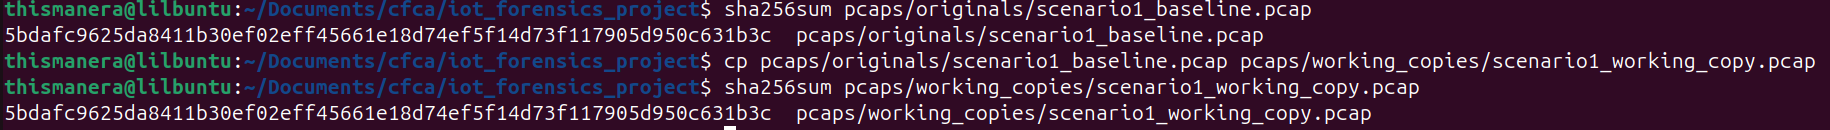
\includegraphics[width=0.85\textwidth]{Images/experiments/terminal_hash_scenario1}
	\caption{Terminal execution demonstrating the SHA-256 hashing and working copy verification.}
	\label{fig:hash_scenario1}
\end{figure}
	
\subsubsection{Baseline Validation and Extracted Metrics}

Following the successful verification of the working copy, the original evidence file was securely isolated to prevent accidental modification. The duplicated working copy was then processed through the Zeek Network Security Monitor (Phase 2). 

Utilizing the \texttt{-C} directive to bypass virtualized checksum offloading errors inherent to the Mininet environment, Zeek successfully parsed the raw binary traffic into structured metadata logs. The resulting artifacts, predominantly the \texttt{conn.log} and \texttt{dns.log}, were exported to a dedicated directory, yielding a clean, noise-reduced dataset ready for ingestion and behavioral analysis.

\begin{figure}[H]
	\centering
	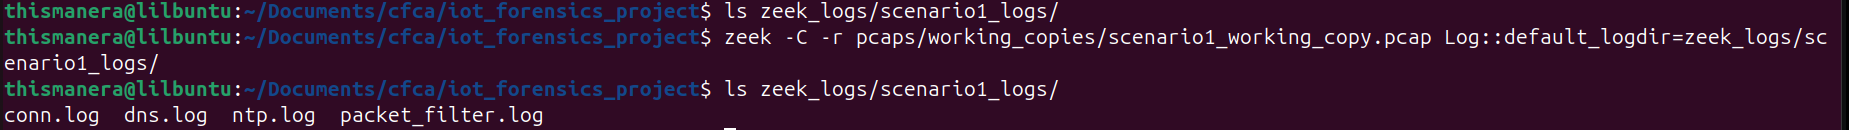
\includegraphics[width=0.85\textwidth]{Images/experiments/zeek_scenario1}
	\caption{Zeek log extraction of Scenario 1.}
	\label{fig:zeekscenario1}
\end{figure}

The resulting Zeek logs were ingested into a Python-based Jupyter Notebook to facilitate the behavioral analysis of the simulation. 

\paragraph{MUD Profile Validation}\mbox{}\\

The primary objective of the baseline scenario analysis is to verify that the simulated IoT devices adhered strictly to their programmed MUD profiles during the simulation execution. By cross-referencing the theoretical behavioral parameters against the empirical Zeek metadata, the operational integrity of the smart home topology can be definitively proven.

The following table compares the expected flows versus the empirical flows. As it can be observed, since it is the baseline scenario, a 100\% accuracy is achieved.

\begin{table}[H]
	\centering
	\renewcommand{\arraystretch}{1.1}
	% Resizebox forces the table to perfectly fit the text width of your page
	\resizebox{\textwidth}{!}{%
		\begin{tabular}{@{}l c c l@{}}
			\toprule
			\textbf{Traffic Classification Profile} & \textbf{Expected Flows} & \textbf{Empirical Flows} & \textbf{Status / Delta} \\ 
			\midrule
			\multicolumn{4}{@{}l}{\textbf{Infrastructure \& Core Services}} \\
			DNS Queries (UDP/53) & 42 & 42 & $\checkmark$ Exact Match \\
			NTP Synchronization (UDP/123) & 6 & 6 & $\checkmark$ Exact Match \\
			\addlinespace
			\multicolumn{4}{@{}l}{\textbf{Smart Thermostat (10.0.0.2)}} \\
			MQTT Keep-Alives (TCP/8883) & 121 & 121 & $\checkmark$ Exact Match \\
			MQTT Telemetry Payloads (TCP/8883) & 5 & 5 & $\checkmark$ Exact Match \\
			\addlinespace
			\multicolumn{4}{@{}l}{\textbf{Smart Camera (10.0.0.1)}} \\
			Video Feed Volumetric Stream (UDP/50005) & 1 & 1 & $\checkmark$ Exact Match \\
			TLS Cloud Telemetry (TCP/443) & 5 & 5 & $\checkmark$ Exact Match \\
			\addlinespace
			\multicolumn{4}{@{}l}{\textbf{Environmental Noise / Unaccounted}} \\
			Background ICMP (Gateway $\rightarrow$ Camera) & 0 & 1 & $\sim$ Minor Hypervisor Noise \\
			\midrule
			\textbf{Total Captured Flows} & \textbf{180} & \textbf{181} & \textbf{100\% Accuracy} \\
			\bottomrule
		\end{tabular}%
	} % End of resizebox
	\caption{Scenario 1: Theoretical Expected Traffic vs. Empirical Zeek Capture Baseline}
	\label{tab:scenario1_baseline}
\end{table}

\textbf{As expected, no attacker activity has been registered.} 

\paragraph{Camera Streaming Bandwidth}\mbox{}\\
For visualization purposes, the network bandwidth was recalculated from bits per second to Kilobytes per minute (KB/min). Given a target bandwidth of 500 KB/s (configured as 4,000 Kbps in the pcap\_generator code), the expected bandwidth is 29,296.88 KB/min. The empirical results demonstrated an average of 27,857.80 KB/min. As seen in the figure below, this variance is entirely attributed to the brief temporal delays required to establish maximum transmission speed at \$t=0\$, as well as the socket teardown phase prior to the 1200-second mark. Excluding these boundary periods, the sustained bandwidth strictly adheres to the expected operational parameters.

\begin{figure}[H]
	\centering
	
\includegraphics[width=0.9\linewidth]{../../iot_forensics_project/figures/scenario1/camera_volumetric_flow}
	\caption{Smart Camera Bandwidth evolution over experiment time (Scenario 1).}
	\label{fig:cameravolumetricflow}
\end{figure}

In addition, the camera directional byte ratio has been calculated. From all the traffic exchanged between the camera and the gateway, 99.9998\% of the traffic has been sent by camera, while the rest are responses from the gateway. This is normal since the camera must act as data flow transmitter.

\paragraph{Thermostat IAT Keep Alives}\mbox{}\\
The temporal delta between consecutive keep-alive messages was calculated to assess baseline stability. While the theoretical expected interval is strictly defined at 10.0 seconds, the empirical results demonstrated a near-perfect mean Inter-Arrival Time (IAT) of 10.0004 seconds. Furthermore, the calculated standard deviation of just 0.5078 seconds proves that the execution overhead of the virtualized environment introduces negligible variance to the device's automated reporting loop.

\begin{figure}[H]
	\centering
	
\includegraphics[width=0.9\linewidth]{../../iot_forensics_project/figures/scenario1/thermostat_iat_distribution}
	\caption{IAT of Smart Thermostat Keep Alive messages (Scenario 1).}
	\label{fig:thermostatiatdistribution}
\end{figure}

In addition, the mean size of the temperature reports generated by the Smart Thermostate has been calculated. The standard size is of 27 bytes. This metric will be important in Scenario 4 since the Thermostat is expected to send multiple packets with a bigger size to simulate it has been infected as a botnet. 

\paragraph{Other Metrics}\mbox{}\\
A interaction heatmap has been developed to track and validate the expected communication patterns between the network's internal nodes. This matrix serves as visual proof of the environment's operational baseline, mapping which cross-node communications are authorized by the Manufacturer Usage Description (MUD) profiles. It should be noted that traffic originating from the gateway (inbound responses) was excluded from this visualization. This methodological scoping decision was made to filter out infrastructure noise, focusing the analytical lens strictly on the behaviors, vulnerabilities, and potential lateral movements of the IoT devices themselves during the attack simulations.

\begin{figure}[H]
	\centering
	
\includegraphics[width=0.9\linewidth]{../../iot_forensics_project/figures/scenario1/topology_traffic_matrix}
	\caption{Empirical interaction heatmap detailing authorized internal network flows (Scenario 1).}
	\label{fig:topologytrafficmatrix}
\end{figure}

Finally, another interesting metric is to track the TCP connection state distribution. In a secure, uncompromised IoT network, TCP sessions must exhibit highly disciplined behavioral patterns. Legitimate devices connect to designated cloud endpoints, execute their application-layer handshakes, and terminate gracefully. Therefore, this baseline metric should be heavily dominated by SF (Normal connection establishment and termination) since all the network traffic flows have been programmed to start and end in the duration of the experiment.

As it can be observed all the connections are correctly finalized as expected.

\begin{figure}[H]
	\centering
	
\includegraphics[width=0.9\linewidth]{../../iot_forensics_project/figures/scenario1/tcp_connection_states}
	\caption{TCP Connection State Distribution (Scenario 1).}
	\label{fig:tcpconnectionstates}
\end{figure}



